%% For double-blind review submission
\documentclass[acmlarge,review,anonymous]{acmart}\settopmatter{printfolios=true}
%% For single-blind review submission
%\documentclass[acmlarge,review]{acmart}\settopmatter{printfolios=true}
%% For final camera-ready submission
%\documentclass[acmlarge]{acmart}\settopmatter{}

%% Note: Authors migrating a paper from PACMPL format to traditional
%% SIGPLAN proceedings format should change 'acmlarge' to
%% 'sigplan,10pt'.


%% Some recommended packages.
\usepackage{booktabs}   %% For formal tables:
                        %% http://ctan.org/pkg/booktabs
\usepackage{subcaption} %% For complex figures with subfigures/subcaptions
                        %% http://ctan.org/pkg/subcaption


% AMS packages
\usepackage{amsmath}
\usepackage{amssymb}
\usepackage{amsthm}
\usepackage{mathtools}
\usepackage{mdwlist}

% Hyper links
\usepackage{url}
\usepackage{hyperref}
\hypersetup{
   colorlinks,
   citecolor=black,
   filecolor=black,
   linkcolor=black,
   urlcolor=black
}

% Miscellaneous
\usepackage{paralist}
\usepackage{graphicx}
\usepackage{epstopdf}
\usepackage{float}
\usepackage{supertabular}

% Code highlighting
\usepackage{listings}
\lstset{%
  basicstyle=\ttfamily\small, % the size of the fonts that are used for the code
  keywordstyle=\sffamily\bfseries,
  captionpos=none,
  columns=flexible,
  lineskip=-1pt,
  keepspaces=true,
  showspaces=false,               % show spaces adding particular underscores
  showstringspaces=false,         % underline spaces within strings
  showtabs=false,                 % show tabs within strings adding particular underscores
  breaklines=true,                % sets automatic line breaking
  breakatwhitespace=true,         % sets if automatic breaks should only happen at whitespace
  escapeinside={(*}{*)},
  sensitive=true
}

\lstdefinestyle{sedel}{
  tabsize=2, % sets default tabsize to 2 spaces
  morekeywords={type,trait,new,def, defrec, if, then, else, new, inherits,
    Trait, let, in},
  morecomment=[l]{--},
  morestring=[b]", % 'b' means inside a string delimiters are escaped by a backslash.
  morestring=[b]',
  literate={->}{{$\rightarrow$}}1 {=>}{{$\Rightarrow$}}1 {/\\}{{$\Lambda$}}1,
}

\lstset{style=sedel}

% Revision tools
\usepackage{xspace}
\usepackage{xcolor}
\usepackage{comment}

%\newcommand{\hltext}[2][gray!40]{\colorbox{#1}{#2}}
%\newcommand{\hl}[2][gray!40]{%
%  \colorbox{#1}{$\displaystyle#2$}}
%\newcommand{\mynotes}[3]{{\color{#2} {\sc #1}: #3}}
%\newcommand\bruno[1]{\mynotes{bruno}{red}{#1}}
%\newcommand\jeremy[1]{\mynotes{jeremy}{blue}{#1}}
%\newcommand\name{{\bf Sedel}\xspace}

\newcommand{\turns}{\vdash}
\newcommand{\oftype}{\!:\!}
\newcommand{\subtype}{<:}
\newcommand{\commonsuper}{\Uparrow}
\newcommand{\commonsub}{\Downarrow}
\newcommand{\disjoint}{*}
\newcommand{\disjointimpl}{*_\textnormal{i}}
\newcommand{\disjointax}{*_\textnormal{ax}}
\newcommand{\subst}[2]{\lbrack #2 := #1 \rbrack~}

\newcommand{\yields}[1]{\highlight{$\; \hookrightarrow #1$}}

\newcommand{\ftv}[1]{\textsf{ftv}(#1)}

\newcommand{\binderspace}{\,}
\newcommand{\appspace}{\;}

\newcommand{\inter}{\&}
\newcommand{\union}{|}
\newcommand{\forr}[2]{\forall #1.\binderspace #2}
\newcommand{\fordis}[3]{\for {(#1 \disjoint #2)} {#3}}
\newcommand{\lam}[2]{\lambda #1.\binderspace #2}
\newcommand{\lamty}[3]{\lam {(#1 \oftype #2)} #3}
\newcommand{\blam}[2]{\Lambda #1.\binderspace #2}
\newcommand{\blamdis}[3]{\blam {(#1 \disjoint #2)} #3}
\newcommand{\mergeop}{,,}
\newcommand{\app}[2]{#1 \; #2}
\newcommand{\tapp}[2]{#1 \appspace #2}
\newcommand{\pair}[2]{(#1, #2)}
\newcommand{\proj}[2]{{\code{proj}}_{#1} #2}
\newcommand{\fst}[1]{\app {\code{fst}} {#1}}
\newcommand{\snd}[1]{\app {\code{snd}} {#1}}
\newcommand{\recordType}[2]{\{ #1 : #2 \}}
\newcommand{\recordCon}[2]{\{ #1 = #2 \}}

\newcommand{\true}{\code{True}}
\newcommand{\tyint}{\code{Int}}
\newcommand{\tybool}{\code{Bool}}
\newcommand{\tychar}{\code{Char}}
\newcommand{\tystring}{\code{String}}

\newcommand{\hltext}[2][gray!40]{\colorbox{#1}{#2}}
\newcommand{\hl}[2][gray!40]{%
  \colorbox{#1}{$\displaystyle#2$}}
\newcommand{\mynotes}[3]{{\color{#2} {\sc #1}: #3}}
\newcommand\bruno[1]{\mynotes{bruno}{red}{#1}}
\newcommand\jeremy[1]{\mynotes{jeremy}{blue}{#1}}
\newcommand\name{{\bf SEDEL}\xspace}
\newcommand{\bname}{$ F_{i} $\xspace}

% Ott includes
\input{sections/miniJS.ott.tex}


\makeatletter\if@ACM@journal\makeatother
%% Journal information (used by PACMPL format)
%% Supplied to authors by publisher for camera-ready submission
\acmJournal{PACMPL}
\acmVolume{1}
\acmNumber{1}
\acmArticle{1}
\acmYear{2017}
\acmMonth{1}
\acmDOI{10.1145/nnnnnnn.nnnnnnn}
\startPage{1}
\else\makeatother
%% Conference information (used by SIGPLAN proceedings format)
%% Supplied to authors by publisher for camera-ready submission
\acmConference[PL'17]{ACM SIGPLAN Conference on Programming Languages}{January 01--03, 2017}{New York, NY, USA}
\acmYear{2017}
\acmISBN{978-x-xxxx-xxxx-x/YY/MM}
\acmDOI{10.1145/nnnnnnn.nnnnnnn}
\startPage{1}
\fi


%% Copyright information
%% Supplied to authors (based on authors' rights management selection;
%% see authors.acm.org) by publisher for camera-ready submission
\setcopyright{none}             %% For review submission
%\setcopyright{acmcopyright}
%\setcopyright{acmlicensed}
%\setcopyright{rightsretained}
%\copyrightyear{2017}           %% If different from \acmYear


%% Bibliography style
\bibliographystyle{ACM-Reference-Format}
%% Citation style
%% Note: author/year citations are required for papers published as an
%% issue of PACMPL.
\citestyle{acmauthoryear}   %% For author/year citations



\begin{document}

%% Title information
\title[\name]{\name: Safe and Expressive Delegation-Based Programming}         %% [Short Title] is optional;
                                        %% when present, will be used in
                                        %% header instead of Full Title.
%%\titlenote{with title note}             %% \titlenote is optional;
                                        %% can be repeated if necessary;
                                        %% contents suppressed with 'anonymous'
%%\subtitle{Subtitle}                     %% \subtitle is optional
%%\subtitlenote{with subtitle note}       %% \subtitlenote is optional;
                                        %% can be repeated if necessary;
                                        %% contents suppressed with 'anonymous'


%% Author information
%% Contents and number of authors suppressed with 'anonymous'.
%% Each author should be introduced by \author, followed by
%% \authornote (optional), \orcid (optional), \affiliation, and
%% \email.
%% An author may have multiple affiliations and/or emails; repeat the
%% appropriate command.
%% Many elements are not rendered, but should be provided for metadata
%% extraction tools.

%% Author with single affiliation.
\author{First1 Last1}
\authornote{with author1 note}          %% \authornote is optional;
                                        %% can be repeated if necessary
\orcid{nnnn-nnnn-nnnn-nnnn}             %% \orcid is optional
\affiliation{
  \position{Position1}
  \department{Department1}              %% \department is recommended
  \institution{Institution1}            %% \institution is required
  \streetaddress{Street1 Address1}
  \city{City1}
  \state{State1}
  \postcode{Post-Code1}
  \country{Country1}
}
\email{first1.last1@inst1.edu}          %% \email is recommended

%% Author with two affiliations and emails.
\author{First2 Last2}
\authornote{with author2 note}          %% \authornote is optional;
                                        %% can be repeated if necessary
\orcid{nnnn-nnnn-nnnn-nnnn}             %% \orcid is optional
\affiliation{
  \position{Position2a}
  \department{Department2a}             %% \department is recommended
  \institution{Institution2a}           %% \institution is required
  \streetaddress{Street2a Address2a}
  \city{City2a}
  \state{State2a}
  \postcode{Post-Code2a}
  \country{Country2a}
}
\email{first2.last2@inst2a.com}         %% \email is recommended
\affiliation{
  \position{Position2b}
  \department{Department2b}             %% \department is recommended
  \institution{Institution2b}           %% \institution is required
  \streetaddress{Street3b Address2b}
  \city{City2b}
  \state{State2b}
  \postcode{Post-Code2b}
  \country{Country2b}
}
\email{first2.last2@inst2b.org}         %% \email is recommended


%% Paper note
%% The \thanks command may be used to create a "paper note" ---
%% similar to a title note or an author note, but not explicitly
%% associated with a particular element.  It will appear immediately
%% above the permission/copyright statement.
\thanks{with paper note}                %% \thanks is optional
                                        %% can be repeated if necesary
                                        %% contents suppressed with 'anonymous'


%% Abstract
%% Note: \begin{abstract}...\end{abstract} environment must come
%% before \maketitle command
\begin{abstract}
This paper presents \name: a new delegation based object-oriented
programming language. Unlike most previous designs for delegation
(and also prototype) based languages, \name is statically typed and
has an expressive polymorphic type system. 
The design of \name and its type systems has two primary goals: 
guaranteeing important \emph{safety} properties; and 
ensuring a high-degree of programming \emph{flexibility}.
In terms of safety \name's type system provides, not only the usual 
type-safety property, but also coherence. The coherence property
ensures that the semantics of \name is unambiguous. In particular 
this property is useful to ensure that programs using 
multiple inheritance remain free of ambiguities. 
In terms of flexibility, the polymorphic type system provides 
an expressive form of polymorphism and intersection types that 
can type-check various delegation-based programs and patterns. 
\end{abstract}


%% 2012 ACM Computing Classification System (CSS) concepts
%% Generate at 'http://dl.acm.org/ccs/ccs.cfm'.
\begin{CCSXML}
<ccs2012>
<concept>
<concept_id>10011007.10011006.10011008</concept_id>
<concept_desc>Software and its engineering~General programming languages</concept_desc>
<concept_significance>500</concept_significance>
</concept>
<concept>
<concept_id>10003456.10003457.10003521.10003525</concept_id>
<concept_desc>Social and professional topics~History of programming languages</concept_desc>
<concept_significance>300</concept_significance>
</concept>
</ccs2012>
\end{CCSXML}

\ccsdesc[500]{Software and its engineering~General programming languages}
\ccsdesc[300]{Social and professional topics~History of programming languages}
%% End of generated code


%% Keywords
%% comma separated list
\keywords{keyword1, keyword2, keyword3}  %% \keywords is optional


%% \maketitle
%% Note: \maketitle command must come after title commands, author
%% commands, abstract environment, Computing Classification System
%% environment and commands, and keywords command.
\maketitle

%% -- Starting Point --


\section{Introduction}

Mainstream statically-typed Object-Oriented Programming (OOP) languages (such as Java,
C++ C\# or Scala) all use a similar programming model based on
classes. For the remainder of the paper this will be referred to as
the \emph{standard model}. The standard model has its roots on the
origins of OOP in the 1960's in the Simula~\cite{} language. 
The standard model essentially provides a \emph{covariant} view of
objects, where the following basic properties are expected:
\bruno{are the two below essentially the same?}

\begin{itemize}

\item {\bf Extensions produce subtypes:} In the standard model, when a 
subclass \emph{extends} a class it automatically becomes a 
\emph{subtype} of the super-class. 

\item{\bf Inheritance and subtyping go along together:}
Class extension does two things at once: it inherits code from the
superclass; and it creates a subtype. In other words inheritance and
subtyping always go along together. 

\end{itemize}

The standard model has been sucessefully being used for over 50 years,
so it clearly has demonstrated its value in practice. In our personal
opinion this success can be attributed to a few things. Firstly,
subtyping and inheritance enable forms of reusability and modularity 
that are not easily or naturally available in languages without such
mechanisms. Secondly, the model is relatively simple and intuitive 
to grasp for programmers. \bruno{more?}

Unfortunatelly the study of the theoretical foundations has
taught us that the story about OOP is not quite so simple. Since the
earliest works on the theory of OOP and subtyping, we have known that 
the covariant view of objects is somewhat simplified. 

Cardelli's work on calculi for OOP has shown, for example, that
functions are not strictly covariant.  A function of type $A \to B$ is
a subtype of another function $C \to D$ when $B$ is a subtype of $D$
and $A$ is a \emph{supertype} of $C$. This means, for example that a
function of type $Cat \to Int$ \emph{cannot not be subtype} of a
function with type $Animal \to Int$ (assumming that $Cat$ is a subtype
of $Animal$). In fact, only the opposite can
happen: $Animal \to Int$ can be a subtype of $Cat \to Int$.  This is
at odds with the covariant view. Mainstream OOP languages such as Java or C\# address this
disturbance of the covariant view by making methods \emph{invariant} on 
their argument types. In other words, if a class $A$ with method $m$
extends a class $B$ with method $m$, then $A.m$ can only override 
$B.m$ if the parameters types in both method signatures are \emph{exactly 
the same}. Thus mainstream OOP languages restrict the natural subtyping of
functions. Various other issues related to covariance are known. 
For example...

Cook et al.'s work on ``\emph{Inheritance is not Subtyping}''~\cite{}
is another example of how the theory of  OOP languages contradicts 
the simple covariant model. As Cook et al. argued inheritance and
subtyping are different relations: subtyping being a relation on types 
and inheritance being a relation on objects. In the standard model 
the subtype relation is based on the inheritance hierarchy. This 
would work very well if extensions would \emph{always} produce 
subtypes. However, as Cook et al.'s work famously demonstrated 
this is not always the case. Following their observations about 
inheritance and subtyping, Cook et al. suggest a programing model 
with the following properties:

\begin{itemize}

\item {\bf Inheritance and subtyping should be decoupled:} 
That is, there should be different mechanisms for class inheritance 
and class/interface subtyping. 

\item {\bf Extensions do not always produce subtypes:} 
There are cases where classes can inherit from other classes without 
producing subtypes. 

\end{itemize}

Therefore Cook et al's model does away with the simple-minded covariant 
view of objects, and proposes a more general model

Despite being proposed almost 30 years ago, and one of the most
famous papers in OOP, Cook et al.'s paper has not had much impact 
on the design of OOP languages. A possible explanation for this 


There are multiple flavours of inheritance. To avoid confusion, since 
the same terminology is often used in the literature to mean different 
things, we use the following 3 terms in this paper:

\begin{itemize}



\item{{\bf Static inheritance:}} Static inheritance refers to what the
  typical model of inheritance in class-based languages. The
  inheritance model is said to be static because when using class
  extension, the extended classes are statically known at compile-type.
Static inheritance is used in languages such as Java, Scala or C\# or
C++\footnote{Note that C++ templates allow the Mixin pattern, which
  enables ...}.

\item{{\bf Mutable Inheritance:}} Prototype-based languages such as 
Javascript or Self allow another model of inheritance, which we call
\emph{mutable inheritance}. In this inheritance model, self references 
can be changed at any point. 

\item{{\bf Dynamic Inheritance:}} Dynamic inheritance is a less well-known 
model which stands in between static and mutable inheritance.
Dynamic inheritance is a model used by some academic delegation 
OOP languages, such as ...  
Unlike the static inheritance model, with dynamic inheritance 
objects can inherits from other objects which are not statically
known. However, unlike mutable inheritance, the self-reference is not 
mutable and cannot be arbitrarely changed at run-time. 

\end{itemize}



\section{A Critique of Mainstream Class-Based OOP}

This section discusses several points about mainstream OOP languages
that work against modularity. 

\subsection{No Contravariant Subtyping on Arguments}

Simple example that illustrates this. Need an example with contravariant arguments

\subsection{No Separation Between Inheritance and Subtyping}

Example: visitors. 

\subsection{No Dynamic Inheritance}

Example: find good example? Design patterns?

\subsection{No Multiple Inheritance of Same Class}

Example: composing Object Algebras (can relate to visitors).

% 
\section{Background}
\label{sec:background}

This section recaps the terminologies~\cite{oliveira2016disjoint,
  alpuimdisjoint} that are used throughout the paper in case the readers are not
familiar with the type system (\bname with some extensions) behind \name. In
particular, we show that \name supports (disjoint) intersection types, the merge
operator, parametric polymorphism and extensible records.

\subsection{(Disjoint) Intersection Types and the Merge Operator}
\label{sec:intersection}

Intersection types date back as early as Coppo et al.'s
work~\cite{coppo1981functional}. Since then researchers have studied
intersection types, and some languages have adopted them in one form or another.

In Java, for examples,
\begin{lstlisting}[language=java]
  interface AwithB extends A, B {}
\end{lstlisting}
introduces a new interface \lstinline$AwithB$ that satisfies the interface of
both \lstinline{A} and \lstinline{B}. In Scala, given two concrete traits, it is
possible to use \textit{mixin composition} to create an object that implements
both traits.
\begin{lstlisting}[language=scala]
  trait A
  trait B
  val newAB : A with B = new A with B
\end{lstlisting}
Scala also allows intersection of type parameters. For example,
\begin{lstlisting}[language=scala]
  def merge[A,B] (x: A) (y: B) : A with B = ...
\end{lstlisting}
uses the anonymous intersection of two type parameters \lstinline{A} and
\lstinline{B}.

However, in Scala it is not possible to dynamically compose two objects. For
example, the following code:
\begin{lstlisting}[language=scala]
  // Invalid Scala code:
  def merge[A,B] (x: A) (y: B) : A with B = x with y
\end{lstlisting}
is rejected by the Scala compiler. The problem is that the \lstinline$with$
construct for Scala expression can only be used to mixin traits or classes, not
arbitrary objects. This limitation essentially puts intersection types in Scala
in a second-class status. Although \lstinline{merge} returns an intersection
type, it is hard to build values with such types.

To address the limitation of intersection types in language like Scala, \name
takes the approach of a particular formulation, where intersection types are
introduced by a \textit{merge operator} (denoted by \lstinline{,,}). As
~\citet{dunfield2014elaborating} has argued, a merge operator adds considerable
expressiveness to a calculus. With the merge operator, it is trivial to
implement the \lstinline{merge} function in \name\footnote{Note that this is not
  the correct definition in \name, see Section~\ref{sec:polymorphism} for
  disjoint quantification.}:
\begin{lstlisting}
  def merge A B (x: A) (y: B) : A & B = x ,, y
\end{lstlisting}
In \name, type variables use capitalized names, while term variables use
lowercase names. In contrast to Scala's expression-level \lstinline{with}
construct, the merge operator \lstinline{,,} allows two arbitrary values to be
merged. The resulting type is an intersection type (\lstinline{A & B} in this
case).

\subsubsection{Incoherence and Disjointness}

Unfortunately the implicit nature of elimination for intersection types built
with a merge operator can lead to incoherence. For a language to be coherent, it
is required that any \textit{valid program} has exactly one
meaning~\cite{reynolds1991coherence}. The naive addition of a merge operator
would allow values of overlapping types to be merged. For example, what should
be the result of the following program, which asks for an integer out of a merge
of two integers:
\begin{lstlisting}
  (1 ,, 2) : Int
\end{lstlisting}
Should the result be 1 or 2?

Following the work of~\citet{oliveira2016disjoint}, in \name, two types can be
merged if and only if they are \textit{disjoint}. Disjointness, in its simplest
form, means that the set of values of both types are disjoint. With the
disjointness requirement, \lstinline{1 ,, 2} is rejected by the type system,
while \lstinline{1 ,, 'c'} is accepted.

As for the above \lstinline{merge} function, since it is a polymorphic function,
it is unknown whether the instantiated types of \lstinline{A} and \lstinline{B}
are disjoint or not. It is still possible that incoherence may occur, as shown
in the following program:
\begin{lstlisting}
  (merge Int Int 1 2) : Int
\end{lstlisting}
To avoid incoherence in such circumstances, \name also employs the notion of
disjoint quantification, as explained in Section~\ref{sec:polymorphism}.

\subsubsection{Parametric Polymorphism and Intersection Types}
\label{sec:polymorphism}

Inspired by the work of~\citet{alpuimdisjoint}, \name uses an extension to
universal quantification called \textit{disjoint quantification}, where a type
variable can be constrained so that it is disjoint with a given type. With
disjoint quantification, the correct version of \lstinline{merge}, which is
accepted in \name, is written as:
\begin{lstlisting}
  def merge A [B * A] (x: A) (y: B) : A & B = x ,, y
\end{lstlisting}

The only difference with the previous version lies in the declaration of the
type parameter \lstinline{B}. The notation \lstinline{B * A} means that the type
variable \lstinline{B} is constrained so that it can only be instantiated with
any type disjoint to \lstinline{A}. Thus the problematic use of
\lstinline{merge} as in \lstinline$merge Int Int 1 2$ is rejected because
\lstinline{Int} is not disjoint with \lstinline{Int}.


\subsection{Extensible Records}
\label{sec:records}

Following~\citet{reynolds1997design} and~\citet{castagna1995calculus}, \name
leverages intersection types to type extensible records. The idea is that a
multi-field record can be encoded as merges of single-field records, and
multi-record types as intersections. Therefore in \name, there are only
single-field record constructs. As such, record operations in \name can occur on
\textit{any} type.

\subsubsection{Record Operations}

To illustrate the various operations on records, we consider a record with three
fields:
\begin{lstlisting}
  {open : Int, high : Int, low : Int}
\end{lstlisting}
Note that this type is just syntactic sugar for:
\begin{lstlisting}
  {open : Int} & {high : Int} & {low : Int}
\end{lstlisting}
That is, a multi-field record type is desugared as intersections of single-field
record types.

\name supports three primitive operations related to records:
\textit{construction} \textit{selection} and \textit{restriction}.
\textit{Extension}, described in many other record systems, is delegated to the
merge operator. Working with records is type-safe: the type system prevents
accessing a field that does not exist.

\paragraph{Record construction.} The usual notation for constructing records
\begin{lstlisting}
  {open = 192, high = 195, low = 189}
\end{lstlisting}
is a shorthand for merges of single-field records
\begin{lstlisting}
  {open = 192} ,, {high = 195} ,, {low = 189}
\end{lstlisting}

\paragraph{Record selection.} Fields are extracted using the dot notation. For
example,
\begin{lstlisting}
  {open = 192, high=195, low= 189}.open
\end{lstlisting}
selects the value of the field labelled \lstinline{open} from the record. Since
records are just merges of terms, we can even select a field that is buried deep
inside a merge, so long as it is present.
\begin{lstlisting}
  ({open = 192} ,, 3 ,, {low = 189}).open
\end{lstlisting}

\jeremy{say something about record restriction}

\paragraph{Record extension} Extension, just like construction, is implemented
with the merge operator. The following example adds a \lstinline{close} field to
the record:
\begin{lstlisting}
  {open = 192, high=195, low=189} ,, {close = 195}
\end{lstlisting}


\begin{comment}
\subsubsection{Restriction via Subtyping}

Unlike most record systems, restriction is not a primitive operation in \name.
Instead, \name uses subtyping for restriction. Combined with disjoint
quantification, we can encode a \lstinline{remove} function that removes a given
field from a record:
\lstinputlisting[linerange=5-5]{../examples/record.txt}% APPLY:linerange=RCD_DEF
\lstinline{remove} takes a value x which contains a record of type
\lstinline${low : Int}$ as well as some extra information of type \lstinline{B}.
The disjointness constraint ensures that the value of type \lstinline{B} does
not contain a record with type \lstinline${low : Int}$. The following examples
shows removing the \lstinline{low} field:
\lstinputlisting[linerange=10-11]{../examples/record.txt}% APPLY:linerange=RCD_EG
\end{comment}


\subsubsection{Disjointness of Records}

Most record calculi forbid duplicate labels in the declarations of record types.
Some allow labels coincide but the last field overrides the previous ones.
Records in \name allow duplicate labels. This is because we adopt a lenient
approach to record disjointness~\cite{alpuimdisjoint}. Of course records with
distinct fields are disjoint naturally. \name accepts duplicate labels as long
as the types of the overlapping fields are disjoint. For example,
\begin{lstlisting}
  {open = 192, high = 195, open = true}
\end{lstlisting}
is allowed in \name. An interesting question arises when we try to select a
duplicate label, say \lstinline{open}. What should be the result? Should it be
192 or \lstinline{true}? Neither choice is satisfying, as with the coherence
problem for merges. Instead \name rejects such expression, and asks for more
type information from the context. Thus the following is accepted because there
is only one \lstinline{open} associated with \lstinline{Int}.
\begin{lstlisting}
  {open = 192, high = 195, open = true}.open + 3
\end{lstlisting}

\section{A Tour of \name}
\label{sec:traits}

This section introduces and showcases the main features of \name. In particular
we focus on \name's native support for \textit{dynamically composable traits}.
Along the way, we also explain briefly various other features of \name.
As a running example, we describe a representation of graphical objects such as
circles, ovals, or buttons. The example is illustrative of typical uses of
JavaScript-style mixins, and it is adapted from an online
tutorial~\footnote{\url{https://javascriptweblog.wordpress.com/2011/05/31/a-fresh-look-at-javascript-mixins/}}.
We will use traits to structure the representation and factor out reusable
components. All code snippets in this and later sections are runnable in our
prototype implementation.


\subsection{Simple Traits}

\name natively supports a simple, yet expressive form of
traits~\cite{scharli2003traits}. Traits provide a mechanism of code reuse in
object-oriented programming, which can be used to model disciplined forms of
multiple inheritance. One interesting aspect about traits is the way conflicting
features that typically arise in multiple inheritance are dealt with. Instead of
automatically resolved by scoping rules, conflicts are, in the case of \name,
detected by the type system, and explicitly resolved by the programmer.
There are three interesting points about \name's traits: 1) they are
\emph{statically typed}; 2) they support \emph{constructors}; and 3)
they support \emph{dynamic inheritance}. The support for such
combination of features is one of the key novelties of \name. This, in
combination with the separation of inheritance and subtyping makes the
trait system particularly flexible and expressive.

In the remainder of this section, we demonstrate various trait features in
\name. A comparison with the traditional trait model can be found in
Section~\ref{sec:related}. The desugaring process of traits is
discussed in Section~\ref{sec:desugar}.

\paragraph{Specifying Traits}
A trait is a collection of related methods that characterize only
a specific perspective of the features of an object. Therefore, compared with
programs using class-based inheritance, programs using traits usually have a large number of
small traits rather than fewer but larger classes. Code reuse with traits is
easier than with classes, since traits are usually shorter and can be
\textit{composed}. % It is the ease of composition that makes traits such a
% appealing language feature: two traits can be freely ``added''
% together.
Trait composition is
a symmetric operation, and trait systems provide conflict detection.

Here is a simple trait \lstinline{point} with its two coordinates \lstinline{x}
and \lstinline{y}\footnote{\name only has floating numbers.}.
\lstinputlisting[linerange=4-7]{../examples/box.txt}% APPLY:linerange=POINT_DEF

%The syntax is very similar to Scala's, with the \lstinline{def} keyword
%beginning a term declaration.

The first thing worth noting is that there are two declarations here.
%At this point the reader may wonder what is the \lstinline{type} declaration
%(\lstinline$Point$) for. 
In mainstream OO languages such as Java, a class declaration such as
\lstinline[language=java]$class C { ... }$ does two things at the same time:

\begin{itemize}
\item Declaring a \textit{template} for creating objects;
\item Declaring a new \textit{type}.
\end{itemize}

In contrast, trait declarations in \name only do the former. Type declarations
are defined separately. For example, the type declaration for \lstinline{Point}
declares the types of the (immutable) fields \lstinline{x} and \lstinline{y}.
Separating the two roles of classes has advantages in terms of flexibility,
although one could argue that it is long-winded sometimes. It is easy enough to
add some syntactic sugar to do the two roles with a single definition, but we
will stick to separate definitions in this paper to illustrate its value.

The trait \lstinline{point} provides a simple example of trait
declarations in \name. The following discussions illustrate 
some fundamental features of \name's traits.

\paragraph{Traits as templates for creating objects} An obvious difference of
traits in \name to many other models of
traits~\cite{scharli2003traits,fisher2004typed,odersky2005scalable} is that they
directly serve as templates for objects. In many other trait models, traits are
complemented by classes, which take the responsibility for object creation. In
particular, most models of traits do not allow constructors for traits. As the
\lstinline{point} definition illustrates, however, traits in \name have a single
constructor, which can have an arbitrary number of arguments.

\paragraph{Trait requirements versus provided functionality}
When modelling a trait there are two important aspects: what are the
\emph{requirements} of a trait; and what is the functionality that a trait
\emph{provides}? The requirements of a trait denote the types/methods that the
trait needs to support defining the functionality the trait provides. The trait
\lstinline{point} requires nothing, and provides implementations for the fields
\lstinline{x} and \lstinline{y}. In \name, the type of \lstinline$self$ denotes
what types/methods are required by a trait. \name uses a syntax (inspired by
Scala self type declarations) where the self-reference is explicitly named and
can optionally be given a type. When there is no type annotation on
\lstinline{self}, this means that the trait requires nothing. In this case the
type of \lstinline{self} is the \emph{top} type. This is different from typical
OO languages, where the default type of a class is the same as the class being
defined.

%The purpose of
%declaring types is to use them for type annotations of the self-reference, and
%creating instances. In the trait literature, a trait usually requires a set of
%methods that server as parameters for the provided behaviour. In \name, the type
%of \lstinline$self$ denotes what methods are required.

\paragraph{Creating objects}
We use the \lstinline{new} keyword to create an object. A difference to other OO
languages is that the \lstinline{new} keyword specifies both the intended type
of the object, and how to construct the object using constructors.
\lstinputlisting[linerange=11-11]{../examples/box.txt}% APPLY:linerange=POINT_TEST

\paragraph{Inheriting traits}
A trait can be extended by inheriting all members of
other traits, and defining additional members. This is, in some sense, similar
to class inheritance in traditional OO languages. Traits can inherit
from one or more traits, provided that
no conflicts arise. The trait \lstinline$circle$ extends
\lstinline{point} with an extra field \lstinline{radius}.
\lstinputlisting[linerange=20-22]{../examples/box.txt}% APPLY:linerange=CIRCLE_DEF

The keyword \lstinline{inherits} is one of the two options in \name to introduce
inheritance. In the above example, the trait \lstinline{circle} inherits from
the trait \lstinline{point} two fields \lstinline{x} and \lstinline{y}
and defined its own field \lstinline{radius}.

\paragraph{Intersection types model subtyping}
The type \lstinline{Circle} is defined as the intersection of the type
\lstinline{Point} and a record type with the field \lstinline{radius}. An
intersection type~\cite{coppo1981functional,pottinger1980type} such as
\lstinline{A & B} contains exactly those values which can be used as values of
type \lstinline{A} and of type \lstinline{B}, and as such, \lstinline{A & B}
immediately introduces a subtyping relation between itself and its two
constituent types \lstinline{A} and \lstinline{B}. In the previous example,
\lstinline{Circle} is, unsurprisingly, a subtype of \lstinline{Point}.

\paragraph{Inheritance and subtyping are separated}
Now it is clear that, unlike the common covariant
model, \name separates the concept of subtyping from inheritance. Those two
concepts are not necessarily entangled, although in this particular example,
inheritance goes along with subtyping.

\subsection{Traits with Requirements and ``Abstract'' Methods}

So far the traits we have seen have no requirements. However, very often it is
necessary to call methods using the self-reference. When this happens
we need to express explicit requirements on the traits. An interesting aspect
of \name's trait model is that there is no need for \emph{abstract
  methods}. Instead, abstract methods can be simulated as requirements 
of a trait. 

In our example, each graphical object can be decomposed into two aspects -- its
geometry and its functions. In case of circles, we already have a trait
\lstinline{circle} representing its geometry. We now proceed to define its
functions by another trait (\lstinline{T} is the top type which has a single
value \lstinline{()}).
\lstinputlisting[linerange=30-34]{../examples/box.txt}% APPLY:linerange=CIRCLE_FNS

\noindent Note how in \lstinline$circleFns$ the type of the self-reference is
\lstinline$Circle$, which declares a \lstinline{radius} field that is needed for
the definitions of the methods in the trait. Note also that the trait itself
does not actually contains a \lstinline{radius} definition. In many other OO
models a similar program could be achieved by having an \emph{abstract} radius
definition. In \name there are no abstract definitions (methods or fields), but
a similar result can be achieved via trait requirements.

Requirements are satisfied at object creation time. When \lstinline$circleFns$
is instantiated and composed with other traits, it must be composed with an
implementation of \lstinline$Circle$. For example:
\lstinputlisting[linerange=38-38]{../examples/box.txt}% APPLY:linerange=CIRCLE_FULL

The object \lstinline{circleWithFns} enables us to call
methods from different traits on a single object.
% , such as % \lstinline{circleWithFns.area()} and \lstinline{circleWithFns.radius}

\paragraph{Composition of traits}
The definition of \lstinline{circleWithFns} also shows the second option to
introduce inheritance, namely by \textit{composition} of traits. Composition of
traits is denoted by the operator \lstinline{&}. Thus \name offers two options
when it comes to inheritance: we can either compose beforehand when declaring
traits (using \lstinline{inherits}), or compose at the object creation point
(using \lstinline{new} and the \lstinline{&} operator).

%Under the hood, inheritance is accomplished by using the \textit{merge operator}
%(denoted by \lstinline{,,}). The merge operator~\cite{dunfield2014elaborating}
%allows two arbitrary values to be merged, with the resulting type being an
%intersection type. 
%For example the type of \lstinline{2 ,, true} is
%\lstinline{Int & Bool}.
\begin{comment}
\paragraph{Mutually dependent traits} When two traits are composed, any two
methods in those two traits can refer to each other via the self-reference. We
say these two traits are \textit{mutually dependent}. The next example, though a
bit contrived, illustrates this point.
\lstinputlisting[linerange=5-12]{../examples/evenOdd.txt}% APPLY:linerange=EVEN_ODD

\noindent By utilizing trait requirements, the \lstinline{isEven} and
\lstinline{isOdd} methods can refer to each other in two different traits.
\end{comment}


\paragraph{Multiple trait inheritance} To further demonstrate multiple
trait inheritance, consider adding buttons. The trait of buttons and its type are:
\lstinputlisting[linerange=43-44]{../examples/box.txt}% APPLY:linerange=BUTTON_DEF

Similarly we define functions for buttons as well.
\lstinputlisting[linerange=48-51]{../examples/box.txt}% APPLY:linerange=BUTTON_FNS

\noindent A round button is made of circle and button, so we have
\lstinline{roundButton} inheriting from both \lstinline{circle} and
\lstinline{button}:
\lstinputlisting[linerange=55-57]{../examples/box.txt}% APPLY:linerange=ROUNDBUTTON_DEF

\noindent Finally we create a round button on the fly and test its functionality
as follows:
\lstinputlisting[linerange=109-112]{../examples/box.txt}% APPLY:linerange=ROUNDBUTTON_TEST

\subsection{Detecting And Resolving Conflicts in Trait Composition}
\label{sec:conflicts}

A common problem in multiple inheritance are conflicts. For example, when
inheriting from two traits that have the same field, then it is unclear which
implementation to choose. There are various approaches to deal with conflicts.
The trait-based approach requires conflicts to be resolved at the level of the
composition by the programmer, otherwise the program is rejected by the type
system.

Below we show how conflicting methods in two traits are detected
and resolved. Let us make an oval shape:
\lstinputlisting[linerange=62-64]{../examples/box.txt}% APPLY:linerange=ASOVAL_DEF

The following trait gets rejected because both \lstinline{asOval} and
\lstinline{circle} have a conflicting \lstinline{radius} field.
\lstinputlisting[linerange=69-71]{../examples/box.txt}% APPLY:linerange=CONFLICT_DEF

\noindent As mentioned in Section~\ref{sec:intro}, \name's type system is based
on intersection types. More concretely, \name uses a type system based on
\emph{disjoint intersection types}~\cite{oliveira2016disjoint}. Disjointness, in
its simplest form, means that the set of values of both types are disjoint. The
above problematic program is ill-typed precisely because both
traits (\lstinline{circle} and \lstinline{asOval}) have the same type for the
\lstinline{radius} field, thus violating the disjointness conditions.

\paragraph{Resolving conflicts}
To resolve the conflict, the programmer needs to explicitly state which
\lstinline{radius} gets to stay. \name provides such a means , the so-called
\textit{exclusion} operator (denoted by \lstinline{\}), which allows one to
avoid a conflict before it occurs. The following is one choice, and is accepted
by \name again.
\lstinputlisting[linerange=77-78]{../examples/box.txt}% APPLY:linerange=CONFLICT_RESOLVE

% \noindent Note that because of the disjointness conditions, the exclusion
% operator is able to pinpoint the exact field given a label and a type.


\subsection{Dynamic Instantiation}

One important difference with traditional traits or classes is that traits in
\name are quite dynamic: we are able to compose traits \textit{dynamically} and
then instantiate them later. This is impossible in traditional OO languages, such
as Java, since classes being instantiated must be known statically. In \name, as
we will explain in Section~\ref{sec:desugar}, traits are just terms: they are
first-class values and can be passed around or returned from other functions.

Circle functions can be extended by another method \lstinline{inCircle},
which tests if a given point lies inside the circle.
\lstinputlisting[linerange=90-92]{../examples/box.txt}% APPLY:linerange=CIRCLE_FNS2

\lstinline{CircleFns2} extends \lstinline{CircleFns} by another method
\lstinline{inCircle}, which is implemented using the \lstinline{norm} method --
distance of a point to the origin. We provide two different norms via two traits.
\lstinputlisting[linerange=82-86]{../examples/box.txt}% APPLY:linerange=NORM_DEF

% as shown in trait \lstinline{circleFns2}, is
% implemented by invoking the \lstinline{norm} method from something of type
% \lstinline{Circle & Norm}. So what is this \lstinline{Norm} type? It consists of
% a single method \lstinline{norm}

To facilitate creating round buttons with different norms baked in, we define a
factory that takes a trait \lstinline$norm$ and produces a round button:
\lstinputlisting[linerange=96-98]{../examples/box.txt}% APPLY:linerange=POINT_FUNC

\noindent Here \lstinline{norm}, which is a trait used in the object creation of
\lstinline{roundButtonFac}, is \emph{parameterized}. To express the
type of such unknown trait \name has a special 
\lstinline{Trait} type constructor, and \lstinline$Trait[Point, Norm]$
denotes the type of traits that conforms to the \lstinline$Norm$ type with dependency
on \lstinline{Point}. This gives us the
flexibility to choose different norms at \emph{run-time}. Below is a
round button that provides \lstinline{inCircle} method with Euclidean norm baked
in.
\lstinputlisting[linerange=102-102]{../examples/box.txt}% APPLY:linerange=ROUNDBUTTON_TEST2

This concludes our running example of presenting graphical objects.

\subsection{Parametric Polymorphism and Disjointness Constraints}
\label{sec:merge-construct}

Upon finishing this tour, let us revisit the problematic \lstinline{merge}
operation. As pointed out in Section~\ref{sec:scala-merge}, intersection types
in Scala are not completely first class, since it is hard to build values of
intersections with unknown components. In \name, however, this is trivial. The
\lstinline{merge} operation discussed in~\ref{sec:scala-merge} can be written as:
\lstinputlisting[linerange=4-4]{../examples/merge.txt}% APPLY:linerange=MERGE_EG

\noindent Firstly \name supports parametric polymorphism, and type variables are
identifiers beginning with uppercase letters. Secondly, from the typing point of
view, the difference between \lstinline{merge} in Scala and \name is that the
type variable \lstinline{B} now has a \emph{disjointness
  constraint}~\cite{alpuimdisjoint}. The notation \lstinline{B * A} means that
the type variable \lstinline{B} can be instantiated to any types that are
disjoint to the type \lstinline{A}. Finally, the value of the intersection type
\lstinline{A & B} is directly built using the \textit{merge construct} (denoted
by \lstinline{,,}). The merge construct~\cite{dunfield2014elaborating} allows
two arbitrary (and possible polymorphic) values to be merged, with the resulting type
being an intersection type.

Disjoint polymorphism~\cite{alpuimdisjoint} sets apart \name
from other OO languages, and enables extensible designs as is elaborated in
Section~\ref{sec:OA}.


\section{A Tour of \name}

This section showcases the novel features of \name, notably its native support
for dynamically composable traits. We demonstrate by two examples that \name
overcomes all those limitations mentioned in Section~\ref{sec:critique}.

All code snippets in this section are runnable in our prototype
implementation.


\subsection{Dynamically Composable Traits}
\label{sec:traits}

\name natively supports a simple, yet expressive form of dynamically composable
traits~\cite{scharli2003traits}. Traits provide a mechanism of code reuse in
object-oriented programming, that can be used as an alternative to multiple
inheritance. One interesting aspect about traits is the way conflicting features
that are typical arise in multiple inheritance are dealt with. Instead of
automatically resolved by scoping rules, conflicts are detected by the type
system, and require programmers to explicitly resolve them. In what follows, we
demonstrate various trait features in \name. A comparison with the traditional
trait model can be found in Section~\ref{sec:discuss}. The desugaring process
from traits to \bname is discussed in Section~\ref{sec:desugar}.

We describe a representation of graphical objects such as circles, ovals, or
buttons as our first running example. The example is adapted from a blog
post\footnote{\url{https://javascriptweblog.wordpress.com/2011/05/31/a-fresh-look-at-javascript-mixins/}}.
We will use traits to structure the representation and factor out reusable
components. Along the way, we also explain briefly how various features in \name
are encoded behind the scene.


\subsubsection{Specifying Traits}

A Trait is, in essential, a collection of related methods that characterize only
a specific perspective of the features of an object. Therefore, compared with
programs using inheritance, programs using traits usually have a large number of
small traits rather than fewer but larger classes. Code reuse with traits is
easier than with classes, since traits are usually shorter and can be
\textit{composed}. It is the ease of composition that makes traits such a
appealing language feature: two traits can be freely ``added'' together (which
is an symmetric operation); and trait systems provide conflict detection, etc.

Here is a simple trait \lstinline{point} with its two coordinates \lstinline{x}
and \lstinline{y}.
\lstinputlisting[linerange=4-8]{../examples/box.txt}% APPLY:linerange=POINT_DEF
The syntax is very similar to Scala's, with the \lstinline{def} keyword
beginning a term declaration.

At this point the reader may wonder what is the \lstinline{type} declaration
(\lstinline$Point$) for. In mainstream OO languages such as Java, a class
declaration such as \lstinline[language=java]$class C { ... }$ does two things
at the same time:

\begin{itemize}
\item Declaring a \textit{template} for creating object;
\item Declaring a new \textit{type}.
\end{itemize}

In contrast, trait declarations in \name only do the former. The purpose of
declaring types is to use them for type annotations of the self-reference, and
creating instances. In the trait literature, a trait usually requires a set of
methods that server as parameters for the provided behaviour. In \name, the type
of \lstinline$self$ denotes what methods are required.

Creating an object is via the \lstinline{new} keyword, a convention in many OO
languages.
\lstinputlisting[linerange=12-12]{../examples/box.txt}% APPLY:linerange=POINT_TEST

\subsubsection{Inheriting Traits}

Traits are extensible. A trait can be extended by inheriting all members of
other traits, and defining additional members. This is, in some sense, similar
to class inheritance in traditional OO languages. However, one difference is
that, a trait can inherit one or more traits without any problems, provided that
there are no conflicts arising (cf. Section~\ref{sec:conflicts}).

To demonstrate that, we create another trait \lstinline$circle$ extending
\lstinline{point} with an extra method \lstinline{radius}.
\lstinputlisting[linerange=18-21]{../examples/box.txt}% APPLY:linerange=CIRCLE_DEF

Note here we use the intersection of type \lstinline{Point} and a record type to
model type \lstinline{Circle}. An intersection
type~\cite{dunfield2014elaborating} such as \lstinline{A & B} contains exactly
those values which can be used as values of type \lstinline{A} and of type
\lstinline{B}. As such, \lstinline{A & B} immediately introduces a subtyping
relation between itself and its two component types \lstinline{A} and
\lstinline{B}. Back to the above example, \lstinline{Circle} is a subtype of
\lstinline{Point}, unsurprisingly.

The keyword \lstinline{inherits} is one of the two options in \name to introduce
inheritance. In the above example, trait \lstinline{circle} inherits from trait
\lstinline{point} two methods \lstinline{x} and \lstinline{y} plus its own
method \lstinline{radius}. Now it is clear that, unlike the common covariant
model, \name separates the concept of subtyping from inheritance -- those two
concepts are not necessarily entangled, though in this particular example,
inheritance goes along with subtyping.

Next we represent buttons in the same way as points. Here are the trait of
buttons and its type:
\lstinputlisting[linerange=47-52]{../examples/box.txt}% APPLY:linerange=BUTTON_DEF

\subsubsection{Traits with Dependencies}

In our example, each graphical object can be decomposed into two aspects -- its
geometry and its functions. In case of circles, we already have a trait
\lstinline{circle} representing its geometry. We now proceed to define its
functions by another trait.
\lstinputlisting[linerange=29-38]{../examples/box.txt}% APPLY:linerange=CIRCLE_FNS

Note how in \lstinline$circleFns$ the type of the self-reference is
\lstinline$Circle$! This is in contrast to a typical object-oriented language,
such as Java, where the self-reference must always be of the same type as the
class being defined. It is this functionality that allows us to express
dependencies between traits: when \lstinline$circleFns$ is instantiated and
composed with other traits, they must be composed with an implementation of
\lstinline$Circle$.
\lstinputlisting[linerange=42-42]{../examples/box.txt}% APPLY:linerange=CIRCLE_FULL

The above line also shows the second option to introduce inheritance, namely by
\textit{composition} of traits. In other words, we can either compose beforehand
when declaring traits (using \lstinline{inherits}), or compose at object
creation point (using \lstinline{new} and \lstinline{&} operator).

Under the hood, inheritance is accomplished by using the \textit{merge operator}
(denoted by \lstinline{,,}). The merge operator~\cite{dunfield2014elaborating}
allows two arbitrary values to be merged, with the resulting type being an
intersection type. For example the type of \lstinline{2 ,, true} is
\lstinline{Int & Bool}. Back to the example, the use of merge enables us to call
methods from different traits on a single object, such as
\lstinline{circleWithFns.area()} and \lstinline{circleWithFns.radius}.

Similarly we define functions for buttons as well.
\lstinputlisting[linerange=56-63]{../examples/box.txt}% APPLY:linerange=BUTTON_FNS

It would be a shame if we cannot make a round button from the existing traits we
have! So here it is, trait \lstinline{roundButton} just inherits everything from
traits \lstinline{circle} and \lstinline{button}:
\lstinputlisting[linerange=67-69]{../examples/box.txt}% APPLY:linerange=ROUNDBUTTON_DEF

Next we add abilities to the round button on the fly and test its functionality
as follows:
\lstinputlisting[linerange=124-127]{../examples/box.txt}% APPLY:linerange=ROUNDBUTTON_TEST



\subsubsection{Detecting And Resolving Conflicts in Trait Composition}
\label{sec:conflicts}

A conflict arises if and only if we combine two traits that have identically
named methods. The traditional approach to resolve conflicts is by method
overriding, automatically done by the type system, whereas the trait-based
approach enforces conflicts be resolved on the level of the composition by the
programmers, otherwise the program is rejected by the type system. The following
example shows how conflicting methods in two traits are detected and resolved.

Let us introduce another shape: something oval.
\lstinputlisting[linerange=74-77]{../examples/box.txt}% APPLY:linerange=ASOVAL_DEF

The following trait gets rejected because both \lstinline{asOval} and
\lstinline{circle} have a conflicting \lstinline{radius} method.
\lstinputlisting[linerange=82-83]{../examples/box.txt}% APPLY:linerange=CONFLICT_DEF

Conflict detecting is one of the selling points of traits. In \name this feature
comes for free because of the requirement that intersection types are
\textit{disjoint}~\cite{oliveira2016disjoint}. Disjointness, in its simplest
form, means that the set of values of both types are disjoint. The above
problematic program fails at passing type checking precisely because both of the
traits (\lstinline{circle} and \lstinline{asOval}) have the same type of the
\lstinline{radius} method, thus violating the disjointness constraint.

To resolve the conflict, the programmer needs to explicitly state which
\lstinline{radius} gets to stay. \name provides such a means , the so-called
\textit{exclusion} operator (denoted by \lstinline{\}), which allows one to
avoid a conflict before it occurs. The following is one choice, and is accepted
by \name again.
\lstinputlisting[linerange=89-90]{../examples/box.txt}% APPLY:linerange=CONFLICT_RESOLVE



\subsection{Dynamic Instantiation}

One difference with traditional traits or classes is that traits in \name are
quite dynamic: we are able to compose traits \textit{dynamically} and then
instantiate them later. This is impossible in traditional OO language, such as
Java, since classes being instantiated must be known statically. In \name, as we
will explain in Section~\ref{sec:desugar}, traits are just terms: they are
first-class values and can be passed around or returned from a function.

Let us extend the functions of circles by another method \lstinline{inCircle},
which, given a point, tests if the point lies inside the circle.
\lstinputlisting[linerange=104-107]{../examples/box.txt}% APPLY:linerange=CIRCLE_FNS2

\lstinline{CircleFns2} just extends \lstinline{CircleFns} by another method
\lstinline{inCircle}, which, as shown in trait \lstinline{circleFns2}, is
implemented by invoking the \lstinline{norm} method from something of type
\lstinline{Circle & Norm}. So what is this \lstinline{Norm} type? It consists of
a single method \lstinline{norm} -- distance of a point to the origin . We
provide two different norms via two traits.
\lstinputlisting[linerange=94-100]{../examples/box.txt}% APPLY:linerange=NORM_DEF

To facilitate creating round buttons with different norms baked in, we define a
factory that takes a trait \lstinline$norm$ and produces a round button:
\lstinputlisting[linerange=111-113]{../examples/box.txt}% APPLY:linerange=POINT_FUNC

Here \lstinline{Trait} is a built-in keyword, and \lstinline$Trait[Point, Norm]$
is the type of traits that conforms to the \lstinline$Norm$ type with dependency
on \lstinline{Point}. It is worth noting that this kind of dynamic composition
and instantiation is impossible in traditional OO languages, such as Java,
because the concrete implementation of \lstinline{norm} is unknown at
compile-time, let alone compose it with other traits. This gives us the
flexibility to choose different norms. For example, below is another version of
round button that provides \lstinline{inCircle} method with Euclidean norm baked
in.
\lstinputlisting[linerange=117-117]{../examples/box.txt}% APPLY:linerange=ROUNDBUTTON_TEST2



\subsection{Extensibility and Subtyping}
\label{sec:extensibility}

Various solutions to the Expression Problem~\cite{wadler1998expression} in the
literature~\cite{finally-tagless,oliveira09modular,DelawareOS13,oliveira2012extensibility,
  swierstra:la-carte} are closely related to type-theoretic encodings of
datatypes. Indeed, variants of the same idea keep appearing in different
programming languages, because the encoding of the idea needs to exploit the
particular features of the programming language (or theorem prover).
Unfortunately language-specific constructs obscure the key ideas behind those
solutions. As our second running example, we presents \name's solution to the
Expression Problem that intends to capture the key ideas of various solutions in
the literature.

To start, we begin with a very simple system modeling arithmetic expressions and
evaluation. The initial system constitutes expressions with two variants
(literals and addition), as depicted below:
\lstinputlisting[linerange=4-7]{../examples/visitor.txt}% APPLY:linerange=ALGEBRA_DEF

The first part, captured by the type \lstinline{ExpAlg[E]}, constitutes the
so-called algebra of the datatype. The first component abstracts over the type
of literal expressions (\lstinline{Int -> E}). The second component abstracts
over the type of addition expression (\lstinline{E -> E -> E}).

The second part, which is the actual type of the arithmetic expression, is:
\lstinputlisting[linerange=11-11]{../examples/visitor.txt}% APPLY:linerange=CHURCH_DEF
An attentive reader may immediately recognize this is exactly the VISITOR
pattern: the method \lstinline{accept} takes an internal visitor as argument.

% \paragraph{Data constructors.} Using \lstinline{Exp} the two data constrcutors
% are defined as follows:
% \lstinputlisting[linerange=52-61]{../examples/visitor.txt}% APPLY:linerange=DC_DEF
% Note that the notation \lstinline{/\E} is type abstraction: it introduces a type
% variable in the environment.


\paragraph{Operations.} Defining operations over expressions requires
implementing \lstinline{ExpAlg[E]}. An interesting operation over expressions is
evaluation. The first step is to choose a suitable concrete type for
instantiating the type parameter \lstinline{E}. One such suitable type is:
\lstinputlisting[linerange=15-15]{../examples/visitor.txt}% APPLY:linerange=EVAL_DEF
Using \lstinline{IEval}, we can define a trait that implements the evaluation
rule for each variant:
\lstinputlisting[linerange=19-22]{../examples/visitor.txt}% APPLY:linerange=EVAL_IMPL


\paragraph{Add a subtraction variant.} Interesting things happen when a new
variant, such as subtraction is added. To do so, we need to extend both
\lstinline{ExpAlg[E]} and \lstinline{evalAlg}:
\lstinputlisting[linerange=27-31]{../examples/visitor.txt}% APPLY:linerange=SUB_DEF
Firstly, \lstinline{SubExpAlg[E]} defines an extended algebra that contains the
variants of the original plus the new subtraction variant. Intersection types
are used to model \textit{type inheritance}. Secondly, a new type of expressions
(\lstinline{ExtExp}) with subtraction is needed. It is important to note that
the \lstinline{accept} method now takes the new algebra \lstinline{SubExpAlg[E]}
as argument.

\paragraph{Inheritance is not subtyping.} In the presence of subtyping, there
are interesting subtyping relations between datatypes and their
extensions~\cite{oliveira09modular}. An interesting aspect about subtyping in
the new system is that subtyping follows the opposite direction of the
extension. In other words, subtyping is contravariant with respect to the
extension. First note that \lstinline{SubExpAlg[E]} appears in parameter
position of \lstinline{accept} and function parameters are naturally
contravariant: \lstinline{ExtExp} should be a \textit{supertype} of
\lstinline{Exp}. By contrast, in common OO languages, type inheritance and
subtyping always go along together. For example, Scala forbids any kind of
type-refinement on method parameter types. The consequence of this is that in
those languages, it is impossible to express that \lstinline{ExtExp} is both an
extension and a supertype of \lstinline{Exp}. Such kind of phenomena is an
example where ``inheritance is not subtyping''~\cite{cook1989inheritance}.

\paragraph{Add a new operation.} The second type of extension is adding a new
operation, such as pretty printing. Similar to evaluation, the interface of the
pretty printing feature is modeled as:
\lstinputlisting[linerange=37-37]{../examples/visitor.txt}% APPLY:linerange=PRINT_DEF
The implementation is spelled out straightforwardly:
\lstinputlisting[linerange=42-46]{../examples/visitor.txt}% APPLY:linerange=PRINT_IMPL


\paragraph{Usage.} The last piece is to define convenient data constructors:
\lstinputlisting[linerange=52-61]{../examples/visitor.txt}% APPLY:linerange=DC_DEF
So now we can test the shiny new system:
\lstinputlisting[linerange=66-70]{../examples/visitor.txt}% APPLY:linerange=VISITOR_EG
Notice that we are able to pass \lstinline{lit 5}, which is of type
\lstinline{Exp}, to \lstinline{sub}, which expects a value of type
\lstinline{ExtExp}. This works precisely because \lstinline{Exp} is a
\textit{subtype} of \lstinline{ExtExp}.



\subsection{How much dynamic is too much}
\label{sec:dynamic}

The solution to the Expression Problem presented in
Section~\ref{sec:extensibility} has one wrinkle in its usage. To be able to call
different operations from the same expression \lstinline{e}, we need to make two
copies \lstinline{o1} and \lstinline{o2}: one is used for printing, while the
other is used for evaluation. An ideal approach would be allowing a single object
to be created that supports both the printing and evaluation features.
Unfortunately, dynamic composition of algebras is non-trivial.
\citet{oliveira2012extensibility} addressed this problem by proposing
\textit{object algebra combinators} that combine multiple algebras into one.
However, as they noted, such combinators written in Java are difficult to use in
practice. A version of this combinator has been encoded in Scala using
intersection types and an encoding of the merge
operator~\cite{oliveira2013feature, rendel14attributes}. Again, the Scala
encoding of the merge operator is quite complex as it relies on low-level
type-unsafe programming features such as dynamic proxies, reflection or other
meta-programming techniques. In \name there is no need for such complex
encoding, as the merge operator is natively supported.

The combinator is defined by the \lstinline{combine} trait, which takes two
algebras to create a combined algebra. It does so by appropriately delegating
behaviours in each component algebra to the combined algebra.

\lstinputlisting[linerange=49-54]{../examples/visitor3.txt}% APPLY:linerange=COMBINE1_DEF

Something new is in the above trait declaration. \name supports parametric
polymorphism. In \name, type variables use uppercase letters. Following the work
of~\citet{alpuimdisjoint}, \name uses an extension to universal quantification
called \textit{disjoint quantification}, where a type variable can be
constrained so that it is disjoint with a given type (\lstinline{B * A} for
example). Parametric polymorphism is need because \lstinline{combine} must
compose algebras with arbitrary type parameters. A disjointness constraint is
needed to ensure that two input algebras build values of disjoint types
(otherwise ambiguity could arise).

With \lstinline{combine} at hand, we can finally have a object \lstinline{o}
print and evaluate at the same time:

\lstinputlisting[linerange=72-75]{../examples/visitor3.txt}% APPLY:linerange=COMBINE1_TEST

An acute reader may have smelled some boilerplate code in the definition of
\lstinline{combine}. After all, \lstinline{combine} just invokes the
corresponding method on the arguments, which is solely driven by the types of
the two input algebras and the resulting algebra. It turns out that the type
system behind \name is powerful enough to derive such definition for us:
\lstinline{combine} is no more than just the merge of two algebras!

\lstinputlisting[linerange=60-60]{../examples/visitor3.txt}% APPLY:linerange=COMBINE_DEF

That's it. No more boilerplate necessary. Two points worth noting: 1) \name
supports \textit{dynamic inheritance}. Notice how we let \lstinline{combine1}
``inherits'' \lstinline{f & g}, for which the implementation is unknown
statically. 2) \name supports multiple inheritance of traits with the same type:
both \lstinline{f} and \lstinline{g} are traits of the subtraction algebra. Type
systems for many OO languages are too inflexible to express this kind of dynamic
inheritance. \name hits a sweet spot in the design space of being how much
dynamic, where we retain as much flexibility as in a dynamic language without
sacrificing the type-safety guarantee we always love from a static type system.


\section{Applications}

% Report on various applications encoded with \name. Conduct a larger case study with visitors.

\jeremy{Example of interpreter using visitor pattern from PAPL, illustrating
  ``inheritance is not subtyping''}

This section shows the expressiveness of \name. We show that features of \name
(dynamically composable traits, intersection types, the merge operator,
parametric polymorphism and disjoint quantification) enable extensible designs
that have been presented in mainstream languages. In particular, \name address
limitations of those languages, making the designs significantly simpler. In
what follows, we preset, in a step-by-step way, a modular interpreter that
supports various operations with various features.



\begin{itemize}
\item Clojure Protocols: http://www.ibm.com/developerworks/library/j-clojure-protocols/
\item Ruby mixin
\item JS mixin
\end{itemize}


\section{Desugaring}
\label{sec:desugar}


The section provides the procedures of desugaring traits to \bname. The idea
behind trait translation is inspired by the functional mixin semantics using
open recursion, which is proposed by~\citet{cook1989denotational} in an untyped
setting. However, our translation is done in the context of a statically-typed
programming language, which is exactly why conflicts can be \textit{statically}
detected in traits.

\subsection{Trait Declarations}

Essentially traits are translated into term declarations, with methods becoming
record fields. The self-reference is adjusted to be the last parameter of the
declaration. For example,
\begin{lstlisting}
  trait point(x : Int, y: Int) { self : Point =>
    def x() = x
    def y() = self.x()
  }
\end{lstlisting}
becomes
\begin{lstlisting}
  def point (x : Int) (y : Int) (self : Point) =
  { x = \_ -> x
  , y = \_ -> self.x()
  }
\end{lstlisting}

Now it is clear that \lstinline{self} is not a special keyword: it can
have any name.

More formally, a trait of the form
\begin{lstlisting}[mathescape=true]
  trait m [$A_1$, ..., $A_n$] ($x_1 : A_1$, ..., $x_n : A_n$) inherits $a_1$ & ... & $a_n$ { s : $A_0$ =>
    def $m_1$(...) = $e_1$
    ...
    def $m_n$(...) = $e_n$
  }
\end{lstlisting}
is translated into a term declaration of the form
\begin{lstlisting}[mathescape=true]
  def m $A_1$ ... $A_n$ $(x_1 : A_1)$ ... $(x_n : A_n)$ $(s : A_0)$ = $a_1$(s) ,, ... ,, $a_n$(s) ,,
  {
    $m_1$ = \(...) -> $e_1$
  , ...
  , $m_n$ = \(...) -> $e_n$
  }
\end{lstlisting}


\subsection{Instantiations of Traits}

\name allows creating a single object from one or more traits. Specifically,
\lstinline{new} instantiates a trait by taking the fixpoint of its
corresponding open term. In fact, \lstinline{new} is translated as an inlined
fixpoint. For example,
\begin{lstlisting}
  new[Point] point(3,4)
\end{lstlisting}
becomes
\begin{lstlisting}
  let self : Point = point 3 4 self in self
\end{lstlisting}
Essentially the open term is closed using \textit{lazy fixpoints}. Lazy
fixpoints are a standard way to encode dynamic mixin inheritance and bind
self-reference in denotational semantics~\cite{cook1989denotational}.

Lazy fixpoints are implemented in \name using the built-in \lstinline{let}
construct (possibly recursive), which employs call-by-name semantics. It is
possible to choose call-by-value, then the type of the self-reference would
becomes a thunk, that is, \lstinline$T -> Point$.

The composition of traits in the \lstinline{new} expression is desugared using
the merge operator. Now it is clear that the reason traits have conflict
detection for free is that the merge operator is enforcing two terms being
merged are disjoint. For example,
\begin{lstlisting}
  new[Point & Norm] point(3,4) & euclideanNorm()
\end{lstlisting}
is turned into
\begin{lstlisting}
  let self : Point & Norm = (point 3 4 self) ,, (euclideanNorm () self) in self
\end{lstlisting}

Formally, a \lstinline{new} expression of the form
\begin{lstlisting}[mathescape=true]
  new[$A_1$ & ... & $A_n$] $a_1$ & ... & $a_n$
\end{lstlisting}
is translated into a let expression of the form
\begin{lstlisting}[mathescape=true]
  let self : $A_1$ & ... & $A_n$ = $a_1$(self) ,, ... ,, $a_n$(self) in self
\end{lstlisting}

\subsection{The Type for Traits}

\lstinline[mathescape=true]{Trait[$T_1, T_2$]} denotes the type of those traits
which provide an interface described by the type $T_2$ with dependency on $T_1$.
In fact, it is just like a type constructor except for the fact that it is
built-in in the language, and that the encoding is not exposed to the
programmers.

Formally, a trait type of the form \lstinline[mathescape=true]{Trait[$T_1, T_2$]} becomes \lstinline[mathescape=true]{$T_1$ -> $T_2$}.

\subsection{Record System}

Following~\citet{reynolds1997design} and~\citet{castagna1995calculus}, \name
leverages intersection types to type extensible records. The idea is that a
multi-field record can be encoded as merges of single-field records, and
multi-record types as intersections. Therefore in \name, there are only
single-field record constructs. As such, record operations in \name can occur on
\textit{any} type.

\subsubsection{Record Operations}

To illustrate the various operations on records, we consider a record with three
fields:
\begin{lstlisting}
  {open : Int, high : Int, low : Int}
\end{lstlisting}
Note that this type is just syntactic sugar for:
\begin{lstlisting}
  {open : Int} & {high : Int} & {low : Int}
\end{lstlisting}
That is, a multi-field record type is desugared as intersections of single-field
record types.

\name supports three primitive operations related to records:
\textit{construction} \textit{selection} and \textit{restriction}.
\textit{Extension}, described in many other record systems, is delegated to the
merge operator. Working with records is type-safe: the type system prevents
accessing a field that does not exist.

\paragraph{Record construction.} The usual notation for constructing records
\begin{lstlisting}
  {open = 192, high = 195, low = 189}
\end{lstlisting}
is a shorthand for merges of single-field records
\begin{lstlisting}
  {open = 192} ,, {high = 195} ,, {low = 189}
\end{lstlisting}

\paragraph{Record selection.} Fields are extracted using the dot notation. For
example,
\begin{lstlisting}
  {open = 192, high=195, low= 189}.open
\end{lstlisting}
selects the value of the field labelled \lstinline{open} from the record. Since
records are just merges of terms, we can even select a field that is buried deep
inside a merge, so long as it is present.
\begin{lstlisting}
  ({open = 192} ,, 3 ,, {low = 189}).open
\end{lstlisting}

\jeremy{say something about record restriction}

\paragraph{Record extension} Extension, just like construction, is implemented
with the merge operator. The following example adds a \lstinline{close} field to
the record:
\begin{lstlisting}
  {open = 192, high=195, low=189} ,, {close = 195}
\end{lstlisting}


\begin{comment}
\subsubsection{Restriction via Subtyping}

Unlike most record systems, restriction is not a primitive operation in \name.
Instead, \name uses subtyping for restriction. Combined with disjoint
quantification, we can encode a \lstinline{remove} function that removes a given
field from a record:
\lstinputlisting[linerange=5-5]{../examples/record.txt}% APPLY:linerange=RCD_DEF
\lstinline{remove} takes a value x which contains a record of type
\lstinline${low : Int}$ as well as some extra information of type \lstinline{B}.
The disjointness constraint ensures that the value of type \lstinline{B} does
not contain a record with type \lstinline${low : Int}$. The following examples
shows removing the \lstinline{low} field:
\lstinputlisting[linerange=10-11]{../examples/record.txt}% APPLY:linerange=RCD_EG
\end{comment}


\subsubsection{Disjointness of Records}

Most record calculi forbid duplicate labels in the declarations of record types.
Some allow labels coincide but the last field overrides the previous ones.
Records in \name allow duplicate labels. This is because we adopt a lenient
approach to record disjointness~\cite{alpuimdisjoint}. Of course records with
distinct fields are disjoint naturally. \name accepts duplicate labels as long
as the types of the overlapping fields are disjoint. For example,
\begin{lstlisting}
  {open = 192, high = 195, open = true}
\end{lstlisting}
is allowed in \name. An interesting question arises when we try to select a
duplicate label, say \lstinline{open}. What should be the result? Should it be
192 or \lstinline{true}? Neither choice is satisfying, as with the coherence
problem for merges. Instead \name rejects such expression, and asks for more
type information from the context. Thus the following is accepted because there
is only one \lstinline{open} associated with \lstinline{Int}.
\begin{lstlisting}
  {open = 192, high = 195, open = true}.open + 3
\end{lstlisting}

\section{Implementation}

The \name prototype implementation is structured around a typed core language
(\bname with some extensions). The main component of the implementation is an
elaborating type-checker, which takes a \bname expression, checks it, and
produces another expression in the target language. The final expression is then
directly executed by an interpreter. We chose call-by-name untyped lambda
calculus as the target language. Since we focus on the implementation, and types
are irrelevant after type checking, untyped lambda calculus is a suitable choice
with minimal syntax. With some simple optimization, the interpreter delivers
reasonably good execution efficiency.

The overall implementation is unremarkable, as it closely follows the semantics
that was presented by~\citet{alpuimdisjoint}. The whole pipeline is shown in
Figure~\ref{fig:pipeline}. The desugaring phase (cf. Section~\ref{sec:desugar})
takes a simple abstract data type (AST) generated by the parser, and returns a
\bname expression. Trait-related constructs disappear after this phase. The
type checking phase then takes a \bname expression from the previous phase, it
infers and checks its type, and in the meantime, produces an expression in the
target language. The type checker is the most involved component in the
pipeline. It contains a (coercive) subtyping procedure and a disjointness
checker, both of which are the most essential parts for \name to work as we
wanted it. The target expression (pure untyped lambda calculus) then enters the
final phase, and is executed by a simple interpreter.

The prototype implementation is written in just 1400 lines of Haskell code.

\begin{figure}
  \centering
  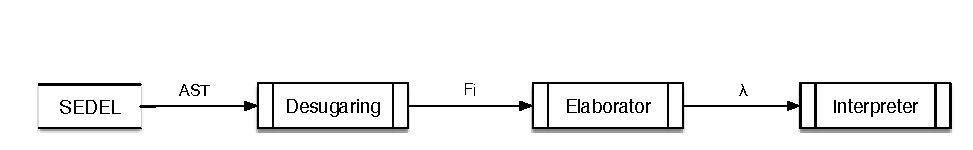
\includegraphics[scale=0.9]{pipeline.eps}
  \caption{The pipeline of \name}
  \label{fig:pipeline}
\end{figure}


\section{Discussion}
\label{sec:discuss}

Discuss the limitations/issues of \name. The differences from the original trait model.

\begin{itemize}
\item Override: Form a new trait by layering additional methods over an existing
  trait. This operation is an asymmetric sum.
\item Exclusion: forms a new trait by removing a method from an existing trait
\end{itemize}


\begin{itemize}
\item Traits have no proper notation of inheritance relationship (no super keyword)
\item Traits have no nice syntax of redefining
\item traits allow annotation of type, then term declarations don't need to
\end{itemize}

\section{Related Work}

\begin{figure}[t]
  \centering
  \begin{tabular}{l|ccccc}
    \hline
     & \bf{Statically typed} & \bf{Polymorphism} & \bf{Covariant model} & \bf{Dynamic inheritance}  \\
    \hline
    \name & \cmark & \cmark & \xmark & \cmark \\
    \hline
    Scala & \cmark & \cmark & \cmark & \xmark \\
    \hline
    Java & \cmark & \cmark & \cmark & \xmark

  \end{tabular}
  \caption{Comparison between \name and various similar languages.}
  \label{fig:comparision}
\end{figure}


\subsection{(Disjoint) Intersection Types, Merge Operator}

There is a large body of work on studying intersection types. Dating back to
works as early as~\citet{coppo1981functional} and~\citet{pottinger1980type},
their motivation was to use intersection types to characterize exactly all
strongly normalizing lambda terms. Forsythe~\cite{reynolds1997design} is
probably the first practical programming language based on intersection types.
Since then various programming languages, including
CDuce~\cite{benzaken2003cduce}, Stardust~\cite{Dunfield07:Stardust}, Microsoft's
TypeScript, Redhat's Ceylon, Facebook's Flow, and Scala~\cite{scala-overview}
have incorporated some notion of intersection types.

The merge operator was first introduced in the Forsythe
language~\cite{reynolds1997design}. Recent work
by~\citet{dunfield2014elaborating} shows significant expressiveness of type
systems with intersection types and a merge operator. However their languages
all lack a important and desirable property of coherence. The limitation was
addressed by~\citet{oliveira2016disjoint}, where they introduce the notion of
disjointness to ensure coherence.

Previous work on incorporating polymorphism with intersection types includes
Pierce's $F_\wedge$~\cite{pierce1991programming2} and the recent work
by~\citet{Castagna:2014}. The former supports intersection types, polymorphism
and, as an extension, the merge operator. However $F_\wedge$ is incoherent due
to the use of such an extension. The latter is a coherent calculus with a
special merge operator that works on functions only. The \bname calculus,
proposed by~\citet{alpuimdisjoint} in their latest work, is the first coherent
calculus that includes parametric polymorphism, intersection types and a merge
operator. \bname serves the theoretical foundation of \name.


\subsection{Mainstream Languages with Delegation Mechanism}

\begin{itemize}
\item Clojure Protocols
  % http://www.ibm.com/developerworks/library/j-clojure-protocols/
\item Ruby mixin
\item JS mixin
\end{itemize}

They are all dynamically typed.

\subsection{Statically typed Delegation-based Languages}

\citet{cook1989inheritance} are the first to propose a typed model of
inheritance where subtyping and inheritance are two separate concepts. In
particular, they introduce the notion of \textit{type inheritance} and show that
inherited objects have inherited types, not subtypes. An interesting aspect of
their model is the \textbf{with} construct, used to join two records. This is
somewhat similar to our merge construct. However two major differences are worth
pointing out: 1) the \textbf{with} construct operates only on records, and 2) it
is a biased operation, meaning the conflict is resolved by favoring values from
its right argument. This is in sheer contrast with \name, where the merge
construct allows merging two arbitrary terms of disjoint types. \jeremy{Cook's
  model uses recursive types and F-bounded polymorphism to type object
  inheritance, while we don't have recursive types.}






\begin{itemize}
\item read ``Inheritance is not subtyping'', notice their ``with'' construct can
  only merge records, problematic to encode the extend operator used in JS style
  mixin, it's also a biased operation.

\item ``mixin-based inheritance''

\item ``Dynamically composable collaborations with delegation layers''

\item ``Type-safe delegation for run-time component adaptation''

\item ``A delegation-based object calculus with subtyping''

\item ``Big Bang Designing a Statically-Typed Scripting Language''

\item ``Building a Typed Scripting Language''
  % https://jscholarship.library.jhu.edu/bitstream/handle/1774.2/39502/PALMER-DISSERTATION-2015.pdf?sequence=1&isAllowed=y

\item ``An imperative, first-order calculus with object extension''

\item ``Object-Oriented Multi-Methods in Cecil''

\end{itemize}

Do they have polymorphic type systems? Do they support mutable self reference?

\subsection{Class-based Languages with More Advanced Form of Inheritance}

\begin{itemize}
\item Eiffel

\item ``Nominal and Structural Subtyping in Component-Based Programming''
\item ``Object-Oriented Composition Untangled''
% \item https://pdfs.semanticscholar.org/7a0a/b7ffce1c1e1195832502d6cb7ace0646596e.pdf
\item ``Engineering a programming language: The type and class system of Sather ''
\end{itemize}



\section{Conclusion}

This paper describes \name: a polymorphic, statically-typed and delegation-based
programming language. \name provides a powerful form of conflict-free multiple
inheritance mechanism called dynamically composable trait. \name is both safe
and flexible. Throughout the paper, we have shown how the mechanisms of \name
improve extensibility design pattern such as Extensible Visitors and Object
Algebras.

There are many avenues for future work. On one hand, we intend to port the core
functionality of \name into a JVM-based compiler. One the other hand, \name is
still very simple, lacking interesting features such as state variables,
recursive types, \textbf{super} keyword, etc. So we are interested to see how
our trait model interacts with those features. Finally we plan to further study
the formal meta-theory of the extended version of \bname.


%% Acknowledgments
\begin{acks}                            %% acks environment is optional
                                        %% contents suppressed with 'anonymous'
  %% Commands \grantsponsor{<sponsorID>}{<name>}{<url>} and
  %% \grantnum[<url>]{<sponsorID>}{<number>} should be used to
  %% acknowledge financial support and will be used by metadata
  %% extraction tools.
  This material is based upon work supported by the
  \grantsponsor{GS100000001}{National Science
    Foundation}{http://dx.doi.org/10.13039/100000001} under Grant
  No.~\grantnum{GS100000001}{nnnnnnn} and Grant
  No.~\grantnum{GS100000001}{mmmmmmm}.  Any opinions, findings, and
  conclusions or recommendations expressed in this material are those
  of the author and do not necessarily reflect the views of the
  National Science Foundation.
\end{acks}


%% Bibliography
\bibliography{paper}


%% Appendix
% \appendix
% \section{Appendix}

% Text of appendix \ldots

\end{document}
